\documentclass{standalone}

% --------------------------------------------------------
% \usepackage{subfigure}
\usepackage{tikz}
\usepackage{subcaption, tkz-tab} 
\usepackage{pgfplots}

%  Colors
\PassOptionsToPackage{table,usenames,dvipsnames*,svgnames,hyperref}{xcolor}
\RequirePackage{xcolor}
% \definecolor{light-gray}{gray}{0.85}
% \definecolor{lighter-gray}{gray}{0.95}
\definecolor{dark-gray}{gray}{0.35}


% --------------------------------------------------------
\usetikzlibrary{calc, decorations.pathreplacing}   %allows coordinate calculations.
\usetikzlibrary{shapes,arrows}
\usetikzlibrary{positioning}
\usetikzlibrary{matrix}
\usetikzlibrary{arrows.meta, calc, fit, tikzmark}

% \usepgflibrary{shapes.multipart, decorations.pathreplacing}
\usepgfplotslibrary{groupplots}
% \pgfplotsset{compat=1.8}
% \pgfplotsset{compat=newest}
\pgfplotsset{compat=1.16}




% --------------------------------------------------------
\begin{document}

% \begin{tikzpicture}
	  \begin{tikzpicture}[domain=0:5,
                      scale=1, thick]

\tikzset{
    % >=stealth'    ,
    pil/.style={ ->, thick, shorten <=0.1pt,  shorten >=0.1pt,},
    dasharrow/.style={ ->, thick, shorten <=1pt,  shorten >=1pt, dashed},
    %Define style for boxes
  }
  \usetikzlibrary{calc}   %allows coordinate calculations.
  \tikzstyle{loosely dashed} = [dash pattern=on 6pt off 6pt]
  \tikzstyle{dasharrow} = [->, thick, shorten <=1pt,  shorten >=1pt, dashed]
% dot/.style={circle,fill=black,minimum size=4pt,inner sep=0pt, outer sep=-1pt},
  %Define linear parameters for supply and demand
    \def\dint{4.5}          %Y-intercept for DEMAND.
    \def\dslp{-0.5}         %Slope for DEMAND.
    \def\sint{2}          %Y-intercept for SUPPLY.
    \def\sslp{0.5}          %Slope for SUPPLY.
    \def\demand{\x,{\dslp*\x+\dint}}
    \def\supply{\x,{\sslp*\x+\sint}}
% Define coordinates.
    \coordinate (ints) at ({(\sint-\dint)/(\dslp-\sslp)},{(\sint-\dint)/(\dslp-\sslp)*\sslp+\sint});
    \coordinate (ep) at  (0,{(\sint-\dint)/(\dslp-\sslp)*\sslp+\sint});
    \coordinate (eq) at  ({(\sint-\dint)/(\dslp-\sslp)},0);
    \coordinate (dint) at (0,{\dint});
    \coordinate (sint) at (0,{\sint});
    % DEMAND
    \draw[thick,color=dark-gray, domain=0.25:5.25] plot (\demand) node[right] {Demand};
    % SUPPLY
    \draw[very thick,color=black, domain=0.25:5.25] plot (\supply) node[right] {Supply};
    % supply going to infinity
    \def\fe{3.25}
    \draw [loosely dashed, color=black] (0.2, \fe) -- (5.5,\fe);
    \filldraw[fill=black, draw=black] (0,\fe) circle (0.1);
    \node[anchor=east] (fe) at (-0.1,\fe)  { $\bar{v}_h$ };
    \node[anchor=south, color=dark-gray] (zeta) at (6,\fe)  { $\zeta \to \infty$};
    \draw[->, bend left=30, draw=dark-gray] (4.6,4.2) to (5.25,\fe+0.1);
    % Draw axes, and dotted equilibrium lines.
    \draw[->] (0,0) -- (6.2,0) node[right] {\Large{ $M_h$ }};   % axes
    \draw[->] (0,0) -- (0,6.2) node[above] {\Large{ $v_h$ }};
  \end{tikzpicture}
  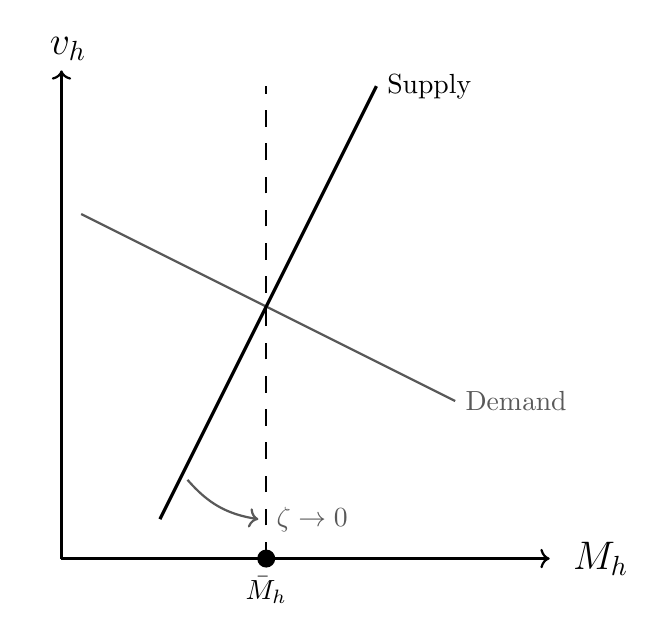
\begin{tikzpicture}[domain=0:5,
                      scale=1,thick]
  \usetikzlibrary{calc}   %allows coordinate calculations.
  \tikzstyle{loosely dashed} = [dash pattern=on 6pt off 6pt]
  \tikzstyle{dasharrow} = [->, thick, shorten <=1pt,  shorten >=1pt, dashed]
  %Define linear parameters for supply and demand
    \def\dint{4.5}          %Y-intercept for DEMAND.
    \def\dslp{-0.5}         %Slope for DEMAND.
    \def\sint{-2}          %Y-intercept for SUPPLY.
    \def\sslp{2}          %Slope for SUPPLY.
    \def\demand{\x,{\dslp*\x+\dint}}
    \def\supply{\x,{\sslp*\x+\sint}}
% Define coordinates.
    \coordinate (ints) at ({(\sint-\dint)/(\dslp-\sslp)},{(\sint-\dint)/(\dslp-\sslp)*\sslp+\sint});
    \coordinate (ep) at  (0,{(\sint-\dint)/(\dslp-\sslp)*\sslp+\sint});
    \coordinate (eq) at  ({(\sint-\dint)/(\dslp-\sslp)},0);
    \coordinate (dint) at (0,{\dint});
    \coordinate (sint) at (0,{\sint});
% DEMAND
    \draw[thick,color=dark-gray, domain=0.25:5] plot (\demand) node[right] {Demand};
% SUPPLY
    \draw[very thick,color=black, domain=1.25:4] plot (\supply) node[right] {Supply};
    \def\Me{2.6}
    \draw [loosely dashed, color=black] (\Me, 0) -- (\Me, 6);
    \filldraw[fill=black, draw=black] (\Me, 0) circle (0.1);
    \node[anchor=north] (me) at (\Me, -0.1)  { $\bar{M}_h$ };
    \node[anchor=west, color=dark-gray] (zeta) at (\Me, 0.5)  { $\zeta \to 0$};
    \draw[->, bend right=20, draw=dark-gray] (1.6,1) to (2.5,0.5);
    % Draw axes, and dotted equilibrium lines.
    \draw[->] (0,0) -- (6.2,0) node[right] {\Large{ $M_h$ }};   % axes
    \draw[->] (0,0) -- (0,6.2) node[above] {\Large{ $v_h$ }};
  \end{tikzpicture}
  
% \end{tikzpicture}


\end{document}
% --------------------------------------------------------